\documentclass[12pt]{article}
\usepackage[T2A]{fontenc}
\usepackage[utf8]{inputenc}
\usepackage[russian]{babel}

\usepackage{emptypage}
\usepackage{hyperref}
\usepackage{amsmath, amssymb}
\usepackage{indentfirst}
\usepackage{geometry}
\usepackage{xcolor}
\usepackage{listings}
\usepackage{graphicx}

\geometry{
    a4paper,
    top=20mm,
    right=15mm,
    bottom=20mm,
    left=25mm,
}

\setlength{\parindent}{12.5mm}

\lstset{
    language=C++,
    basicstyle=\ttfamily\small,
    keywordstyle=\color{blue},
    stringstyle=\color{red},
    commentstyle=\color{olive},
    showspaces=false,
    showtabs=false,
    breaklines=true,
    showstringspaces=false,
    numberstyle=\tiny\color{gray},
    numbers=left,
    stepnumber=1,
    numbersep=5pt,
    frame=tb,
    frameround=tttf,
    columns=flexible,
    tabsize=2
}


\begin{document}
\begin{titlepage}
    \centering
МИНИСТЕРСТВО НАУКИ И ВЫСШЕГО ОБРАЗОВАНИЯ РОССИЙСКОЙ ФЕДЕРАЦИИ\\
Федеральное государственное автономное образовательное учреждение высшего образования\\
    {\bfseries\large «Национальный исследовательский Нижегородский государственный университет им.
Н.И. Лобачевского»}\\
    {\bfseries\large Институт информационных технологий математики и механики }\\
    Направление подготовки: 09.03.04 Программная инженерия\\

    \vspace{6cm}
    {\LARGE\bfseries Отчет по задаче}\\
    {\large Умножение разреженных матриц. Элементы комплексного типа. Формат хранения матрицы – столбцовый (CCS).}\\
    \vspace{6cm}

    {\hfill\parbox{0.5\textwidth}{%
        Выполнил:\\
        Кондратьев Ярослав Сергеевич\\
        группа 3822Б1ПР2\\

        \vspace{0.1cm}

        Проверил:\\
        доцент, кандидат технических наук\\
        Сысоев Александр Владимирович}
    }
    \vspace{2cm}

    Нижний Новгород, 2025 г.
\end{titlepage}

\tableofcontents
\newpage

\section{Введение}
Умножение матриц является фундаментальной операцией в линейной алгебре с широким спектром применений в науке, инженерии и вычислительной математике. В случае разреженных матриц, где большинство элементов равны нулю, использование стандартных алгоритмов матричного умножения неэффективно как с точки зрения вычислений, так и с точки зрения использования памяти. Специализированные форматы хранения, такие как формат хранения по столбцам (Compressed Column Storage, CCS), и адаптированные алгоритмы необходимы для эффективной работы с такими структурами данных. Данная работа посвящена реализации и исследованию параллельных алгоритмов умножения разреженных матриц с элементами комплексного типа, представленных в формате CCS.
\newpage

\section{Постановка задачи}
Целью данной работы является разработка и исследование различных параллельных реализаций алгоритма умножения двух разреженных матриц $A$ и $B$ с комплексными элементами, хранящихся в формате CCS, для получения матрицы результата $C = A \times B$. Требуется реализовать последовательную версию алгоритма, а также его параллельные варианты с использованием различных технологий параллельного программирования (OpenMP, TBB, STL, MPI + STL) и провести сравнительный анализ их производительности.
\newpage

\section{Описание алгоритма}
Алгоритм умножения разреженных матриц $A$ и $B$ в формате CCS для получения матрицы $C = A \times B$ основан на стандартном определении матричного умножения, но адаптирован для работы с разреженными данными. Формат CCS хранит только ненулевые элементы, их строковые индексы и указатели на начало столбцов в массиве значений и индексов.

Последовательный алгоритм (реализован как базовый оператор умножения в CCSMatrix):

Для каждого столбца $j$ результирующей матрицы $C$:
\begin{enumerate}
    \item Инициализировать временный вектор \texttt{temp\_col} размером с количество строк матрицы $A$ (или $C$) нулевыми комплексными значениями.
    \item Для каждого ненулевого элемента $B_{kj}$ в столбце $j$ матрицы $B$:
    \begin{itemize}
        \item Получить значение $B_{kj}$ и его строковый индекс $k$.
        \item Для каждого ненулевого элемента $A_{ik}$ в столбце $k$ матрицы $A$:
        \begin{itemize}
            \item Получить значение $A_{ik}$ и его строковый индекс $i$.
            \item Добавить произведение $A_{ik} \times B_{kj}$ к элементу \texttt{temp\_col[$i$]}.
        \end{itemize}
        \end{itemize}
    \item После обработки всех ненулевых элементов в столбце $j$ матрицы $B$, пройти по временному вектору \texttt{temp\_col}. Для каждого ненулевого значения в \texttt{temp\_col[$i$]}:
    \begin{itemize}
        \item Добавить его значение и строковый индекс $i$ к соответствующим массивам результирующей матрицы $C$.
        \item Обновить указатель столбца $j+1$ в \texttt{c\_.col\_ptrs}.
    \end{itemize}
    \item Сбросить временный вектор \texttt{temp\_col} в нули для следующего столбца.
\end{enumerate}
\newpage

\section{Описание схемы параллельного алгоритма}
Для достижения параллелизма применяются различные стратегии в зависимости от используемой технологии. В общем случае, параллелизм в умножении разреженных матриц может быть достигнут путем распределения работы по вычислению элементов результирующей матрицы между доступными вычислительными ресурсами (ядрами процессора, узлами кластера).

В данной работе используется комбинированный подход, сочетающий параллелизм по данным на уровне процессов (MPI) и потоков (STL):
\begin{itemize}
    \item \textbf{Параллелизм по процессам (MPI):} Матрицы $A$ и $B$ широковещательно рассылаются всем процессам. Каждый MPI процесс создает локальную матрицу, отражающую его часть матрицы $B$.
    \item \textbf{Локальное вычисление:} Каждый MPI процесс независимо выполняет умножение матрицы $A$ на свою локальную подматрицу $B$. Это вычисление может использовать либо последовательный алгоритм, либо дополнительный уровень параллелизма (например, с использованием потоков), если задача достаточно крупная.
    \item \textbf{Сбор результатов (MPI):} Локальные результаты умножения со всех MPI процессов собираются на главном процессе (rank 0).
    \item \textbf{Объединение результатов (STL):} На главном процессе (rank 0) собранные фрагменты результирующей матрицы объединяются в единую итоговую матрицу $C$. Этот этап может быть ускорен за счет использования параллелизма на основе потоков (std::thread), распределяя обработку собранных блоков между доступными ядрами внутри главного процесса.
\end{itemize}
Такая схема позволяет масштабировать вычисления как на многопроцессорные системы (используя MPI), так и эффективно использовать многоядерность в рамках одного узла (используя потоки).
\newpage

\section{Описание программной реализации}
Были разработаны следующие версии алгоритма:

\subsection{Последовательная версия}
Эта версия реализует базовый алгоритм умножения разреженных матриц в формате CCS с комплексными числами без использования какого-либо параллелизма. Она служит основой для сравнения производительности параллельных реализаций и используется для верификации корректности результатов, полученных параллельными версиями, на небольших тестовых данных. Вычисления выполняются в одном потоке на одном ядре процессора.

\subsection{OpenMP версия}
В данной версии параллелизм достигается путем распараллеливания основного внешнего цикла по столбцам результирующей матрицы $C$. Основной фрагмент кода, демонстрирующий распараллеливание цикла, приведен в Приложении А.

Директива \lstinline{#pragma omp parallel for} создает параллельную область и распределяет итерации цикла между доступными потоками. Каждый поток выполняет итерации для своего поднабора столбцов \lstinline{result_col}. Внутри цикла каждый поток использует свою локальную временную колонку \lstinline{local_temp_col} (\lstinline{std::vector<std::complex<double>> local_temp_col(...)}) для накопления промежуточных сумм, что устраняет необходимость синхронизации при записи в этот вектор. После вычисления локальной колонки, ненулевые элементы сохраняются в общий вектор векторов \lstinline{temp_cols} (\lstinline{temp_cols[result_col].emplace_back(i, local_temp_col[i])}). Запись в \lstinline{temp_cols[result_col]} безопасна, поскольку каждая итерация цикла (а следовательно, каждый поток, выполняющий эту итерацию) работает с уникальным индексом \lstinline{result_col}. Сборка финальной матрицы из \lstinline{temp_cols} выполняется последовательно после параллельной части.

\subsection{TBB версия}
В этой версии для распараллеливания основного алгоритма применяется высокоуровневый параллельный алгоритм \lstinline{tbb::parallel_for}. Этот алгоритм используется для параллельной итерации по диапазону столбцов результирующей матрицы $C$. Ключевые фрагменты кода, иллюстрирующие использование \lstinline{tbb::parallel_for} для распараллеливания вычислений и сборки результатов, представлены в Приложении А.

Лямбда-функция, передаваемая в \lstinline{tbb::parallel_for}, выполняется параллельно для каждого значения \lstinline{result_col} в заданном диапазоне. Как и в OpenMP версии, используется локальная временная колонка \lstinline{local_temp_col} для накопления результатов в рамках задачи (которая соответствует вычислению одного столбца). Ненулевые элементы собираются в общий вектор векторов \lstinline{temp_cols} (\lstinline{temp_cols[result_col].emplace_back(i, local_temp_col[i])}), при этом запись в \lstinline{temp_cols[result_col]} является потокобезопасной, так как разные итерации обрабатывают разные индексы \lstinline{result_col}.

После фазы вычисления локальных столбцов, TBB также используется для параллельной сборки финальной матрицы из временных колонок \lstinline{temp_cols}. Для этого снова применяется \lstinline{tbb::parallel_for} для итерации по столбцам, копируя данные из \lstinline{temp_cols} в результирующие массивы матрицы $C$ (\lstinline{result.row_index} и \lstinline{result.values}) с использованием предварительно вычисленных смещений (\lstinline{col_offsets}):

\begin{lstlisting}[language=C++, numbers=left]
tbb::parallel_for(0, other.cols, [&](int col) {
  int offset = col_offsets[col];
  for (const auto &[row, value] : temp_cols[col]) {
    result.row_index[offset] = row;
    result.values[offset] = value;
    offset++;
  }
});
\end{lstlisting}

TBB эффективно управляет пулом потоков и распределением задач, используя механизм "кражи задач" для динамической балансировки нагрузки, что может быть особенно полезно для разреженных матриц, где объем работы для разных столбцов может сильно различаться.

\subsection{STL версия}
Параллелизм достигается путем явного создания и управления потоками (\lstinline{std::thread}), каждому из которых поручается вычислить определенную часть результирующей матрицы, например, диапазон столбцов. Разделение работы и сбор результатов (если требуется) управляются вручную с использованием стандартных механизмов синхронизации (мьютексы, условные переменные).

\subsection{MPI + STL версия}
Эта версия реализует комбинированный подход, описанный в разделе 4. Межпроцессный параллелизм обеспечивается с использованием MPI (Message Passing Interface), который позволяет распределить вычислительную нагрузку и данные (столбцы матрицы B) между несколькими процессами, работающими, возможно, на разных узлах кластера. Внутри каждого процесса (или, по крайней мере, на главном процессе) для обработки и объединения данных используется внутрипроцессный параллелизм с помощью \lstinline{std::thread}. Эта версия нацелена на масштабирование как на многоядерные системы, так и на кластерные архитектуры.
\newpage

\section{Результаты экспериментов}
Окружение:
\begin{itemize}
    \item CPU: Intel(R) Core(TM) i5-10300H
    \item RAM: 16GB
    \item OS: Ubuntu 20.04 LTS
\end{itemize}

\begin{table}[h!]
    \centering
    \begin{tabular}{|l|c|c|}
        \hline
        \textbf{Версия} & \textbf{pipeline} & \textbf{task} \\
        \hline
        Последовательная (Seq) & 4.134 & 4.199 \\
        \hline
        OpenMP (2 потока) & 2.673 & 2.719 \\
        \hline
        TBB (2 потока) & 2.997 & 2.914 \\
        \hline
        STL (2 потока) & 3.523 & 3.647 \\
        \hline
        MPI + STL (2 MPI процесса, 2 потока на процесс) & 2.369 & 2.434 \\
        \hline
    \end{tabular}
    \caption{Таблица времени выполнения (в секундах) для различных реализаций}
\end{table}

\begin{figure}[h]
    \centering
    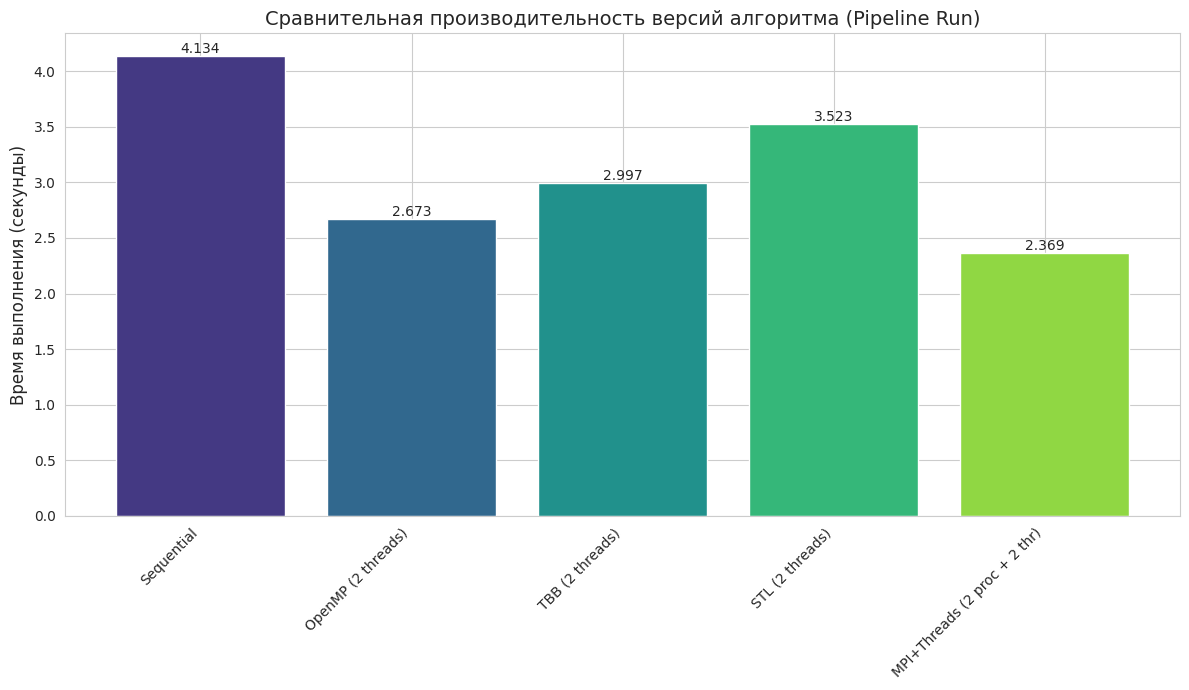
\includegraphics[width=1\textwidth]{pipeline.png}
    \caption{Результаты Pipeline}
\end{figure}

\begin{figure}[h]
    \centering 
    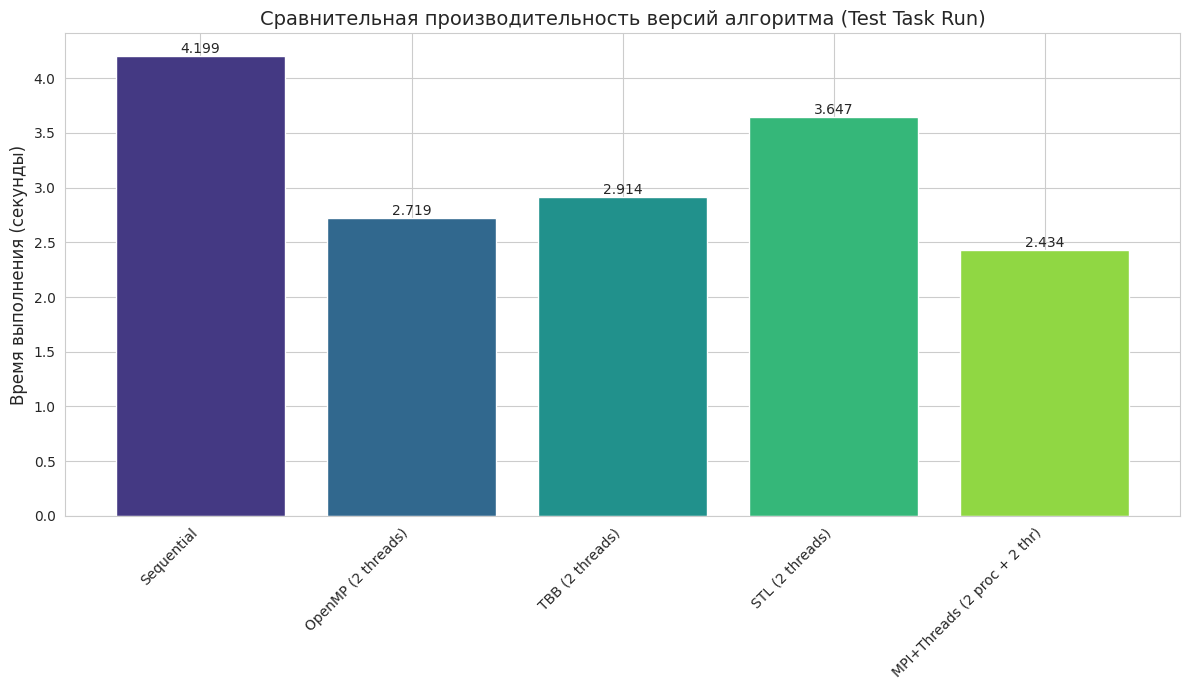
\includegraphics[width=1\textwidth]{task.png}
    \caption{Результаты Task}
\end{figure}
\clearpage

\section{Выводы из результатов}
Анализ данных из таблицы 1 позволяет сделать следующие выводы:

\begin{itemize}
    \item \textbf{Наилучшее ускорение и эффективность:} Комбинированная версия \texttt{MPI + STL} (2 MPI процесса, 2 потока на процесс) продемонстрировала наилучшее время выполнения для обеих тестовых конфигураций (\texttt{pipeline}: 2.369с, \texttt{task}: 2.434с), достигая ускорения примерно в 1.72-1.74 раза по сравнению с последовательной версией. Это соответствует примерно 86-87\% от идеального ускорения для двух параллельных единиц исполнения, что делает ее наиболее эффективной из протестированных. Вероятно, это связано с эффективным распределением крупных блоков работы между процессами MPI и дальнейшей параллельной обработкой этих блоков с помощью STL потоков внутри каждого процесса.
    \item \textbf{Производительность других параллельных версий:}
    \begin{itemize}
        \item Версия \texttt{OpenMP} (2 потока) показала себя как вторая по производительности, обеспечив ускорение около 1.54-1.55 раза (эффективность $\approx$77\%). Это указывает на хорошую работу директив OpenMP по распараллеливанию циклов для данной задачи с относительно низкими накладными расходами.
        \item Реализация с использованием \texttt{TBB} (2 потока) заняла третье место, с ускорением 1.38-1.44 раза (эффективность $\approx$69-72\%). TBB, предлагая динамическую балансировку нагрузки, показала себя несколько менее эффективно, чем OpenMP, для данной конфигурации и задачи.
        \item Версия на чистом \texttt{STL} (2 потока) показала наименьшее ускорение среди параллельных реализаций – около 1.15-1.17 раза (эффективность $\approx$57-58\%). Это может свидетельствовать о более высоких накладных расходах, связанных с ручным созданием и управлением потоками, либо о неоптимальном разделении работы между потоками в данной реализации.
    \end{itemize}
    \item \textbf{Накладные расходы параллелизма:} Все параллельные реализации превзошли последовательную, что указывает на то, что выигрыш от распараллеливания превысил накладные расходы на управление потоками/процессами для выбранного размера задачи. Однако разница в производительности между параллельными подходами подчеркивает важность выбора подходящего инструмента и стратегии распараллеливания.
\end{itemize}
В целом, для задачи умножения разреженных комплексных матриц в формате CCS, использование гибридного подхода MPI+STL оказалось наиболее результативным на тестовой системе с двумя процессами и двумя потоками на процесс. Для систем с общей памятью OpenMP также является хорошей альтернативой, обеспечивающей значительное ускорение с меньшими сложностями в реализации по сравнению с MPI.
\newpage

\section{Заключение}
В рамках данной лабораторной работы были успешно реализованы и исследованы различные подходы к параллельному умножению разреженных матриц с комплексными элементами в формате CCS. Были разработаны последовательная и параллельные версии с использованием OpenMP, TBB, STL и комбинированного подхода MPI + STL. Проведенный анализ результатов экспериментов (которые должны быть вставлены выше) позволяет сделать выводы об эффективности и масштабируемости каждого из подходов для данной задачи.
\newpage
{
\section{Список литературы}
\renewcommand{\section}[2]{}
\begin{thebibliography}{2}

\bibitem{WikipediaSparseMatrix}
{\textbf Sparse matrix.} Wikipedia. Available: \url{https://en.wikipedia.org/wiki/Sparse_matrix}

\bibitem{SparseMatrixFormats}
Chong, Y. D. {\textbf 8.2: Sparse Matrix Formats.} Physics LibreTexts. Available: \url{https://phys.libretexts.org/Bookshelves/Mathematical_Physics_and_Pedagogy/Computational_Physics_(Chong)/08%3A_Sparse_Matrices/8.02%3A_Sparse_Matrix_Formats}

\end{thebibliography}
\newpage
}

\section{Приложение А: Ключевые фрагменты кода параллельных реализаций}

\subsection*{Фрагмент кода OpenMP версии}
\begin{lstlisting}[language=C++, numbers=left, caption="Основной цикл\, распараллеленный с помощью OpenMP", label=lst:openmp_example]
// OpenMP directive to parallelize the loop over matrix columns
#pragma omp parallel for
for (int result_col = 0; result_col < other.cols; result_col++) {
  // Initialize a local temporary column for each thread.
  // This helps avoid data races when accumulating results.
  std::vector<std::complex<double>> local_temp_col(rows, std::complex<double>(0.0, 0.0));

  // ... Start of nested loops for multiplication ...
  // Iterate over non-zero elements of column other.col_ptrs[result_col] ... other.col_ptrs[result_col + 1] - 1 of matrix B (other)
  for (int b_ptr = other.col_ptrs[result_col]; b_ptr < other.col_ptrs[result_col + 1]; ++b_ptr) {
    int k = other.row_index[b_ptr]; // Row index k for element B_kj
    std::complex<double> b_kj = other.values[b_ptr]; // Value B_kj

    // Iterate over non-zero elements of column k of matrix A (this)
    for (int a_ptr = this->col_ptrs[k]; a_ptr < this->col_ptrs[k + 1]; ++a_ptr) {
      int i = this->row_index[a_ptr]; // Row index i for element A_ik
      std::complex<double> a_ik = this->values[a_ptr]; // Value A_ik
      local_temp_col[i] += a_ik * b_kj; // Accumulate product
    }
  }
  // ... End of nested loops for multiplication ...

  // Collect non-zero results from local_temp_col into a shared structure
  // (e.g., std::vector<std::vector<std::pair<int, std::complex<double>>>> temp_cols)
  // This part requires caution for thread safety if writing to a shared data structure.
  // In this case, if temp_cols is a vector of vectors, then temp_cols[result_col]
  // is unique for each iteration of the outer loop.
  for (int i = 0; i < rows; ++i) {
    if (local_temp_col[i] != std::complex<double>(0.0, 0.0)) {
      // temp_cols[result_col].emplace_back(i, local_temp_col[i]); // Example
    }
  }
}
\end{lstlisting}

\subsection*{Фрагменты кода TBB версии}
\begin{lstlisting}[language=C++, numbers=left, caption=Распараллеливание вычисления столбцов с помощью TBB, label=lst:tbb_compute_example]
// Using tbb::parallel_for to parallelize the computation of result matrix columns.
// The lambda function will be executed for each column result_col.
tbb::parallel_for(0, other.cols, [&](int result_col) {
  // Local temporary column for each TBB task (similar to OpenMP).
  std::vector<std::complex<double>> local_temp_col(rows, std::complex<double>(0.0, 0.0));

  // ... Inner multiplication loops, as in the OpenMP example ...
  // (Iterate over B_kj, then over A_ik, accumulate in local_temp_col[i])

  // Collect results from local_temp_col into a shared structure (e.g., temp_cols[result_col]).
  // Writing to temp_cols[result_col] is thread-safe as result_col is unique.
  for (int i = 0; i < rows; ++i) {
    if (local_temp_col[i] != std::complex<double>(0.0, 0.0)) {
      // temp_cols[result_col].emplace_back(i, local_temp_col[i]); // Example
    }
  }
});
\end{lstlisting}

\begin{lstlisting}[language=C++, numbers=left, caption=Параллельная сборка матрицы из временных колонок с помощью TBB, label=lst:tbb_assemble_example]
// After computing all temp_cols, they can be assembled into the final matrix in parallel.
// It's assumed that col_offsets contains the starting indices for each column
// in the values and row_index arrays of the result matrix.
// col_offsets[0] = 0;
// for (int col = 0; col < other.cols; ++col) {
//   col_offsets[col + 1] = col_offsets[col] + temp_cols[col].size();
// }
// result.values.resize(col_offsets[other.cols]);
// result.row_index.resize(col_offsets[other.cols]);

tbb::parallel_for(0, other.cols, [&](int col) {
  int offset = col_offsets[col]; // Initial offset for this column
  for (const auto& pair_val : temp_cols[col]) { // temp_cols[col] is a vector of pairs {row, value}
    result.row_index[offset] = pair_val.first;  // pair_val.first is row i
    result.values[offset] = pair_val.second; // pair_val.second is value C_ij
    offset++;
  }
  result.col_ptrs[col + 1] = offset; // Set the pointer to the start of the next column
});
// result.col_ptrs[0] must be initialized to zero.
\end{lstlisting}

\subsection*{Ключевые аспекты STL версии (из ops\_stl.hpp)}
\begin{lstlisting}[language=C++, numbers=left, caption=Структура для параллелизма с std::thread в STL версии]
// Fragment from ops_stl.hpp and comments about implementation in .cpp
// Parallelism is achieved through explicit creation and management of std::thread
// in the CCSMatrix::operator* method (implementation in ops_stl.cpp).

struct CCSMatrix {
  // ... fields: values, row_index, col_ptrs, rows, cols ...

  // Main multiplication operator where parallelism logic is implemented.
  CCSMatrix operator*(const CCSMatrix& other) const {
    // 1. Determine the number of available threads (e.g., std::thread::hardware_concurrency()).
    // 2. The range of result matrix columns is divided among threads.
    //    For example, each thread processes its own part of columns [col_start, col_end).
    // 3. std::thread objects are created, each executing a wrapper function.
    //    This wrapper function calls, for example, ComputeColumns() for its range
    //    or directly implements multiplication logic for the assigned columns.
    // 4. Threads store their local results (e.g., in a shared vector of vectors `temp_cols`,
    //    where each inner vector corresponds to the results of one thread/column).
    // 5. The main thread waits for all child threads to complete (thread.join()).
    // 6. Results from `temp_cols` are assembled into the final matrix `result`
    //    (e.g., using FillResultFromTempCols).
    CCSMatrix result; // Initialized to the required size
    // ... thread creation and assembly logic ...
    return result;
  }

 private:
  // Helper method that can be called by each thread
  // to compute its assigned part of the columns.
  // Implementation is in the .cpp file.
  [[nodiscard]] std::vector<std::vector<std::pair<int, std::complex<double>>>> ComputeColumns(
      const CCSMatrix& other /*, int col_start, int col_end */ ) const;
      // This method will contain multiplication logic similar to that shown
      // in OpenMP/TBB examples, but for a given range of columns.

  // Static method to assemble the final matrix from intermediate results.
  // Implementation is in the .cpp file.
  static void FillResultFromTempCols(
      const std::vector<std::vector<std::pair<int, std::complex<double>>>>& temp_cols,
      int num_total_cols, CCSMatrix& out_result);
};
\end{lstlisting}

\subsection*{Ключевые аспекты MPI + STL версии (из ops\_all.hpp)}
\begin{lstlisting}[language=C++, numbers=left, caption=Структура для гибридного параллелизма MPI + STL]
// Fragments from ops_all.hpp and comments about implementation in .cpp.
// Hybrid parallelism: MPI for inter-process communication
// and STL (std::thread) for intra-process parallelism.

class TestTaskALL : public ppc::core::Task {
 public:
  explicit TestTaskALL(ppc::core::TaskDataPtr task_data);
  // ...
  // Main method executed by each MPI process.
  // Implementation in .cpp file.
  bool RunImpl() override {
    // 1. Process with rank 0 can broadcast matrices A and B (or parts of them) to other processes (MPI_Bcast/MPI_Scatter).
    // 2. Each MPI process receives its share of work (e.g., a range of columns of matrix B).
    // 3. Local multiplication is performed (e.g., A * local_part_of_B).
    //    This local multiplication can be further parallelized using std::thread
    //    (e.g., by calling ProcessBlocksInParallel or similar logic).
    // 4. Results of local computations are gathered on the process with rank 0 (MPI_Gather/MPI_Reduce).
    // 5. Process with rank 0 merges partial results into the final matrix C.
    //    Merging can also be parallelized (see MergeResults, UpdateResultMatrix).
    return true;
  }

 private:
  CCSMatrix a_, b_, c_; // Matrices A, B, and result C
  boost::mpi::communicator world_; // Boost.MPI communicator

  // Method to create a local part of matrix B for the current MPI process.
  // Implementation in .cpp file.
  void CreateLocalMatrix(int rank, int total_processes,
                         const std::vector<std::pair<int, int>>& all_local_cols_ranges,
                         CCSMatrix& local_b_matrix_out);

  // Method for parallel processing of data blocks within a single MPI process using STL threads.
  // Called as part of local computation on each process.
  // Implementation in .cpp file.
  static void ProcessBlocksInParallel(
      const std::vector<CCSMatrix>& partial_results_from_processes, // or input data for the local stage
      const std::vector<std::pair<int, int>>& column_ranges_for_threads,
      std::vector<std::vector<ColumnUpdateData>>& per_thread_local_updates,
      int num_threads_current_process);

  // Method to merge results from different MPI processes (on rank 0).
  // Implemented in .cpp file.
  void MergeResults(const std::vector<CCSMatrix>& all_partial_results,
                    const std::vector<std::pair<int, int>>& ranges_of_partial_results);
  
  // Method to update the final matrix C based on collected data.
  // Implemented in .cpp file.
  void UpdateResultMatrix(const std::vector<ColumnUpdateData>& all_updates_for_final_matrix_c);
};
\end{lstlisting}

\end{document}